\documentclass[10pt,twocolumn]{article}
\usepackage[a4paper,margin=18mm,columnsep=6.5mm]{geometry}
\usepackage[T1]{fontenc}
\usepackage{lmodern}
\usepackage{microtype}
\usepackage{amsmath,amssymb}
\usepackage{booktabs}
\usepackage{array}
\usepackage{xcolor}
\usepackage{tikz}
\usepackage{pgfplots}
\usepackage{pgfplotstable}
\usepackage{caption}
\usepackage[hidelinks]{hyperref}
\usepackage{balance}
\usepackage{titlesec}
\usetikzlibrary{arrows.meta,positioning,calc,fit,backgrounds}
\pgfplotsset{compat=1.18}
\usepgfplotslibrary{groupplots}

\definecolor{ink}{HTML}{1F2933}
\definecolor{ours}{HTML}{0B6E4F}
\definecolor{rival}{HTML}{C8553D}
\definecolor{third}{HTML}{3D5A80}
\definecolor{soft}{HTML}{E8EEF2}
\definecolor{softgreen}{HTML}{DDEFE6}
\definecolor{softred}{HTML}{F7E3DD}
\definecolor{softblue}{HTML}{DFE7F2}
\definecolor{softgold}{HTML}{F6EBCF}

\captionsetup{font=small,labelfont=bf,skip=5pt}
\titleformat{\section}{\normalfont\large\bfseries}{\thesection}{0.6em}{}
\titleformat{\subsection}{\normalfont\normalsize\bfseries}{\thesubsection}{0.6em}{}
\titlespacing*{\section}{0pt}{10pt plus 2pt}{4pt}
\titlespacing*{\subsection}{0pt}{7pt plus 2pt}{3pt}
\setlength{\parskip}{0pt}
\renewcommand{\arraystretch}{1.08}
\raggedbottom

% Generated by make_data.py. Do not edit.
\newcommand{\setApxm}{68{,}064{,}254}
\newcommand{\setAbpp}{7.964}
\newcommand{\setAtenwins}{23}
\newcommand{\setAten}{70{,}976{,}488}
\newcommand{\setAtengain}{4.28}
\newcommand{\setAtenbpp}{8.305}
\newcommand{\setAninewins}{24}
\newcommand{\setAnine}{72{,}479{,}607}
\newcommand{\setAninegain}{6.49}
\newcommand{\setAninebpp}{8.481}
\newcommand{\setAflifwins}{24}
\newcommand{\setAflif}{75{,}167{,}788}
\newcommand{\setAflifgain}{10.44}
\newcommand{\setAflifbpp}{8.795}
\newcommand{\setAwebpwins}{24}
\newcommand{\setAwebp}{79{,}889{,}788}
\newcommand{\setAwebpgain}{17.37}
\newcommand{\setAwebpbpp}{9.348}
\newcommand{\setApngwins}{24}
\newcommand{\setApng}{106{,}803{,}378}
\newcommand{\setApnggain}{56.92}
\newcommand{\setApngbpp}{12.497}
\newcommand{\setAenc}{16.6}
\newcommand{\setAdec}{12.4}
\newcommand{\setBpxm}{65{,}361{,}460}
\newcommand{\setBbpp}{7.697}
\newcommand{\setBtenwins}{24}
\newcommand{\setBten}{68{,}163{,}312}
\newcommand{\setBtengain}{4.29}
\newcommand{\setBtenbpp}{8.027}
\newcommand{\setBninewins}{24}
\newcommand{\setBnine}{69{,}902{,}596}
\newcommand{\setBninegain}{6.95}
\newcommand{\setBninebpp}{8.232}
\newcommand{\setBflifwins}{24}
\newcommand{\setBflif}{71{,}658{,}973}
\newcommand{\setBflifgain}{9.63}
\newcommand{\setBflifbpp}{8.439}
\newcommand{\setBwebpwins}{24}
\newcommand{\setBwebp}{77{,}229{,}826}
\newcommand{\setBwebpgain}{18.16}
\newcommand{\setBwebpbpp}{9.095}
\newcommand{\setBpngwins}{24}
\newcommand{\setBpng}{106{,}540{,}568}
\newcommand{\setBpnggain}{63.00}
\newcommand{\setBpngbpp}{12.547}
\newcommand{\setBenc}{19.4}
\newcommand{\setBdec}{12.5}
\newcommand{\setCpxm}{69{,}787{,}409}
\newcommand{\setCbpp}{8.110}
\newcommand{\setCtenwins}{24}
\newcommand{\setCten}{72{,}312{,}784}
\newcommand{\setCtengain}{3.62}
\newcommand{\setCtenbpp}{8.404}
\newcommand{\setCninewins}{24}
\newcommand{\setCnine}{73{,}965{,}237}
\newcommand{\setCninegain}{5.99}
\newcommand{\setCninebpp}{8.596}
\newcommand{\setCflifwins}{24}
\newcommand{\setCflif}{76{,}261{,}753}
\newcommand{\setCflifgain}{9.28}
\newcommand{\setCflifbpp}{8.863}
\newcommand{\setCwebpwins}{24}
\newcommand{\setCwebp}{81{,}290{,}848}
\newcommand{\setCwebpgain}{16.48}
\newcommand{\setCwebpbpp}{9.447}
\newcommand{\setCpngwins}{24}
\newcommand{\setCpng}{110{,}420{,}020}
\newcommand{\setCpnggain}{58.22}
\newcommand{\setCpngbpp}{12.832}
\newcommand{\setCenc}{15.0}
\newcommand{\setCdec}{11.4}
\newcommand{\cgeo}{3.66}
\newcommand{\cgeolo}{2.91}
\newcommand{\cgeohi}{4.44}
\newcommand{\cminsave}{0.44}
\newcommand{\cmaxsave}{8.13}
\newcommand{\cslowest}{23.7}
\newcommand{\cslowestdec}{16.9}
\newcommand{\tilecostA}{0.26}
\newcommand{\kfinal}{6{,}750{,}776}
\newcommand{\kbefore}{9{,}818{,}812}
\newcommand{\kpaq}{6{,}649{,}818}
\newcommand{\kfinalbpp}{5.723}
\newcommand{\kbeforebpp}{8.324}
\newcommand{\kpaqbpp}{5.637}
\newcommand{\kdrop}{31.2}
\newcommand{\kpaqgap}{1.52}
\newcommand{\kpaqgapbefore}{47.66}
\newcommand{\kpaqwins}{5}
\newcommand{\kpaqvsjxl}{33.6}
\newcommand{\kmodetwo}{24}
\newcommand{\ksharelo}{84.5}
\newcommand{\ksharehi}{93.9}
\newcommand{\kshare}{87.3}
\newcommand{\dfinal}{2{,}251{,}773}
\newcommand{\dbestname}{JPEG XL e10}
\newcommand{\dbestgain}{9.4}
\newcommand{\dbestwins}{16}
\newcommand{\sppxmwholeenc}{47.8}
\newcommand{\sppxmwholedec}{32.08}
\newcommand{\sppxmtwoenc}{17.2}
\newcommand{\sppxmtwodec}{10.59}
\newcommand{\sppxmfourenc}{8.4}
\newcommand{\sppxmfourdec}{5.73}
\newcommand{\spjxltenenc}{42.0}
\newcommand{\spjxltendec}{0.08}
\newcommand{\spjxlnineenc}{1.8}
\newcommand{\spjxlninedec}{0.08}
\newcommand{\spflifenc}{14.3}
\newcommand{\spflifdec}{0.95}
\newcommand{\spwebpenc}{10.0}
\newcommand{\spwebpdec}{0.07}
\newcommand{\decodegap}{141}
\newcommand{\tilecosttwo}{0.18}
\newcommand{\tilefactor}{3.3}
\newcommand{\play}{5.03}
\newcommand{\playA}{5.04}
\newcommand{\playB}{5.03}
\newcommand{\playC}{5.03}
\newcommand{\playD}{5.03}
\newcommand{\plax}{1.89}
\newcommand{\plaxA}{1.95}
\newcommand{\plaxB}{1.79}
\newcommand{\plaxC}{1.99}
\newcommand{\plaxD}{1.85}
\newcommand{\plaz}{1.14}
\newcommand{\plazA}{1.14}
\newcommand{\plazB}{1.06}
\newcommand{\plazC}{1.22}
\newcommand{\plazD}{1.14}
\newcommand{\plcx}{4.56}
\newcommand{\plcxA}{4.57}
\newcommand{\plcxB}{4.57}
\newcommand{\plcxC}{4.56}
\newcommand{\plcxD}{4.56}
\newcommand{\plcy}{0.57}
\newcommand{\plcyA}{0.52}
\newcommand{\plcyB}{0.36}
\newcommand{\plcyC}{0.77}
\newcommand{\plcyD}{0.66}
\newcommand{\plcz}{0.53}
\newcommand{\plczA}{0.44}
\newcommand{\plczB}{0.32}
\newcommand{\plczC}{0.74}
\newcommand{\plczD}{0.64}
\newcommand{\matrixdecodes}{245}
\newcommand{\latKpairs}{1{,}453}
\newcommand{\latKxmin}{-42}
\newcommand{\latKxmax}{2}
\newcommand{\latKymin}{-21}
\newcommand{\latKymax}{23}
\newcommand{\latOpairs}{11{,}756}
\newcommand{\latOxmin}{-27}
\newcommand{\latOxmax}{17}
\newcommand{\latOymin}{-11}
\newcommand{\latOymax}{33}

\makeatletter\let\rawinput\@@input\makeatother

\pgfplotsset{
  every axis/.append style={font=\footnotesize, tick style={ink!60}, axis line style={ink!60}, label style={font=\footnotesize}, legend style={font=\scriptsize, draw=none, fill=none}},
}
\tikzset{
  box/.style={draw=ink!70, rounded corners=2pt, fill=#1, align=center, font=\scriptsize, inner sep=3.2pt, minimum height=6.5mm},
  box/.default=soft,
  flow/.style={-{Stealth[length=2mm]}, ink!75, line width=0.55pt},
}

\title{\vspace{-8mm}\Large\bfseries What Images Remember:\\Exact Colour Differences and Reproducible Floating Point\\in a Context-Mixing Lossless Image Codec}
\author{Saksham\\[1pt]\normalsize The Truepix project}
\date{November 2026}

\begin{document}
\newcommand{\frontmatter}{%
\maketitle
\vspace{-7mm}
\begin{center}
\begin{minipage}{0.9\textwidth}
\small
\textbf{Abstract.}
A general-purpose compressor, paq8px, is \kpaqvsjxl\% smaller than JPEG~XL on the Kodak benchmark, far beyond what its modelling advantage achieves elsewhere. We show why. About nine tenths of the gap between paq8px and our predictive codec lies in colour rather than brightness, and the cause is historical: the Kodak images are Photo~CD scans whose RGB values are a stretched integer lattice of PhotoYCC samples. A fixed-point inverse places \kshare\% of pixels on a lattice covering 12.8\% of colours, with gains matching Kodak's published constants. Exploiting it cuts our Kodak total by \kdrop\%, to \kfinalbpp\ bits per pixel. Because that gain says nothing about other photographs, we then generalise: hashed contexts over exact colour differences learn such structure with no knowledge of its origin. The resulting codec, Truepix, combines online least squares, parametric models and logistic mixing. On 24 unseen DIV2K images it is \setCtengain\% smaller in total than JPEG~XL at effort~10 and smaller on all 24 (Wilcoxon $p=1.2\times10^{-7}$; geometric-mean lead \cgeo\%, 95\% CI [\cgeolo, \cgeohi]). Two earlier hold-out sets gave leads of \setAtengain\% and \setBtengain\%. Truepix uses floating point yet is reproducible: seven builds across compilers, 32- and 64-bit x86 and WebAssembly wrote byte-identical files, and all \matrixdecodes\ cross-build decodes were exact. It remains far slower than JPEG~XL, and paq8px still compresses more.
\end{minipage}
\end{center}
\vspace{4mm}
}
\twocolumn[\frontmatter]

\section{Introduction}

Lossless image compression has two very different leaders. Standardised codecs such as JPEG~XL \cite{jpegxl} decode in milliseconds. Context-mixing compressors such as paq8px \cite{mahoney,paq8px} are smaller and take minutes. We set out to build a codec between them, and hit an anomaly at once. On the 24-image Kodak suite \cite{kodak}, our codec trailed paq8px by \kpaqgapbefore\%, yet it trailed by only about 8\% on other images. An unexplained gap that large suggests that something is hidden in the data rather than missing from the model.

The explanation turned out to be useful in three ways. It exposes a colour lattice in the most widely used image compression benchmark. It leads to a simple general mechanism that needs no knowledge of how a lattice arose. And it forced a discipline we recommend: once a set has been studied it is spent, so each claim below is tied to a set that was unseen when the codec was frozen.

\paragraph{Contributions.}
\begin{itemize}\setlength\itemsep{1pt}\setlength\parskip{0pt}
\item A diagnosis of the paq8px gap on Kodak, tracing it to the Photo~CD PhotoYCC lattice, verified against Kodak's published conversion (\S\ref{sec:kodak}).
\item Exact-difference contexts, which learn colour lattices online without any parametric fit (\S\ref{sec:exact}).
\item A floating-point context-mixing codec with reproducible output across builds, and the rules that make it so (\S\ref{sec:portable}).
\item Three hold-out evaluations, including the negative results (\S\ref{sec:results}).
\end{itemize}

\section{Related work}

Predictive coding runs from JPEG-LS \cite{jpegls} and CALIC \cite{calic} to the far stronger adaptive schemes built on local least squares \cite{edp}, such as TMW \cite{tmw}, MRP \cite{mrp} and Vanilc \cite{vanilc}. FLIF \cite{flif} and JPEG~XL \cite{jpegxl} offer practical progressive and fast coding. PAQ \cite{mahoney} introduced logistic mixing of many context models, and paq8px \cite{paq8px} carries specialised image models. Learned codecs such as L3C \cite{l3c} replace hand-built models with neural networks.

Recovering a processing history from pixels is well established. Fan and de~Queiroz detect JPEG history and estimate quantisers from bitmaps \cite{fan}, Neelamani et al.\ estimate the colour transform, subsampling and quantisers of decoded colour images and show that this aids recompression \cite{neelamani}, and Lewis and Kuhn study exact JPEG recompression \cite{lewis}. The JPEG side of our lattice work is therefore not new. We found no report of the Photo~CD lattice in the Kodak suite, though our search was limited and we do not claim priority. Reproducible floating point is a known hazard \cite{monniaux,ieee}.

\section{Why paq8px wins on Kodak}
\label{sec:kodak}

\subsection{Where the bits go}

We first split the gap. Each codec compressed the green plane alone, and the remainder of its whole-image size was attributed to colour. Figure~\ref{fig:gap} shows the result for four images: green accounts for only about a tenth of the gap. At that stage Truepix spent about 2.2 and 2.1 bits per pixel on red and blue of \texttt{kodim01} once green was known, while paq8px spent about 1.5 on both together.

\begin{figure}[t]
\centering
\resizebox{\columnwidth}{!}{%
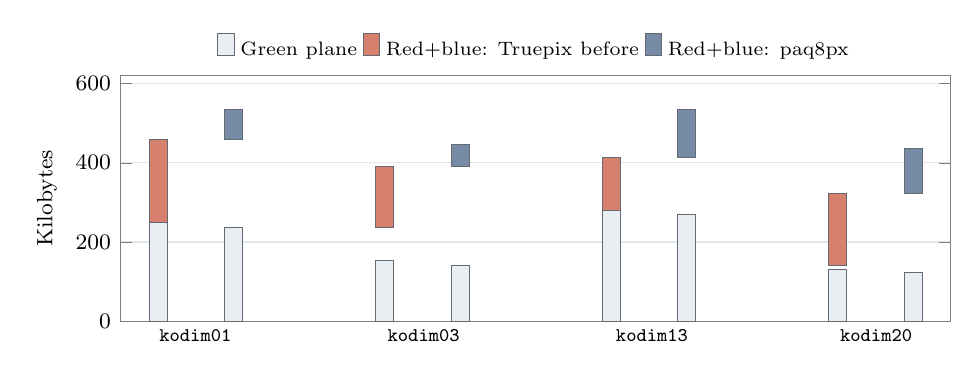
\begin{tikzpicture}
\begin{axis}[
  width=\columnwidth, height=47mm, ybar stacked, bar width=6.5pt,
  symbolic x coords={01a,01b,g1,03a,03b,g2,13a,13b,g3,20a,20b},
  xtick={01a,03a,13a,20a}, xticklabels={},
  ymin=0, ymax=620, ylabel={Kilobytes}, enlarge x limits=0.05, ymajorgrids, grid style={ink!12},
  legend style={at={(0.5,1.02)},anchor=south,legend columns=3}, xtick style={draw=none},
  extra description/.code={
    \foreach \x/\t in {0.09/01,0.365/03,0.64/13,0.91/20}{\node[font=\scriptsize] at (axis description cs:\x,-0.06) {\texttt{kodim\t}};}
  }]
\addplot[fill=soft,draw=ink!70] coordinates {(01a,249.909)(01b,236.361)(03a,154.472)(03b,140.910)(13a,280.043)(13b,270.150)(20a,129.819)(20b,123.459)};
\addplot[fill=rival!75,draw=ink!70] coordinates {(01a,209.649)(03a,153.473)(13a,259.297)(20a,182.611)};
\addplot[fill=third!70,draw=ink!70] coordinates {(01b,74.562)(03b,56.602)(13b,120.603)(20b,111.656)};
\legend{Green plane, Red+blue: Truepix before, Red+blue: paq8px}
\end{axis}
\end{tikzpicture}}
\caption{Size split for the diagnosis, using the codec as it stood before this work. In each pair the left bar is Truepix and the right bar is paq8px. Green is nearly level; colour is not.}
\label{fig:gap}
\end{figure}

\subsection{A lattice in the colour differences}

The colour differences $(R-G,\,B-G)$ are strikingly sparse. Image \texttt{kodim01} uses only \latKpairs\ distinct pairs in 393,216 pixels, while the 262,144-pixel reference photograph \texttt{astronaut} uses \latOpairs. Plotting occupancy reveals why (Figure~\ref{fig:lattice}): Kodak's pairs sit on a skewed grid.

\begin{figure}[t]
\centering
\begin{tikzpicture}
\begin{groupplot}[group style={group size=2 by 1, horizontal sep=9mm}, width=45mm, height=45mm, enlargelimits=false, axis on top, xlabel={$B-G$}, tick label style={font=\scriptsize}, title style={font=\footnotesize, yshift=-1mm}]
\nextgroupplot[title={\texttt{kodim01}}, ylabel={$R-G$}]
\addplot graphics[xmin=\latKxmin,xmax=\latKxmax,ymin=\latKymin,ymax=\latKymax] {data/lattice_kodak.png};
\nextgroupplot[title={\texttt{astronaut}}]
\addplot graphics[xmin=\latOxmin,xmax=\latOxmax,ymin=\latOymin,ymax=\latOymax] {data/lattice_ordinary.png};
\end{groupplot}
\end{tikzpicture}
\caption{Occupancy of colour-difference pairs in a window around each image's median, with darker meaning more pixels. Kodak falls on a lattice; the reference image shows no such grid in this window.}
\label{fig:lattice}
\end{figure}

A two-dimensional Fourier transform of this occupancy gives the lattice with no prior knowledge. Over four images its strongest frequencies were $(0.1348,-0.3994)$ and $(-0.3848,0.0625)$ cycles per level. Inverting them gives the basis vectors in Table~\ref{tab:constants}, which match the steps implied by Kodak's published PhotoYCC decoding \cite{pcd045}:
\begin{align}
L &= 1.3584\,Y, \notag\\
C_1 &= 2.2179\,(c_1-156), \quad C_2 = 1.8215\,(c_2-137), \notag\\
R &= L + C_2,\quad B = L + C_1, \notag\\
G &= L - 0.194\,C_1 - 0.509\,C_2. \label{eq:pcd}
\end{align}
One step of $c_2$ moves $R-G$ by $1.8215\times1.509=2.749$, the $\approx$3-level jump visible in raw pixels. The same document explains the image size, since Photo~CD Base images are $512\times768$, with chroma subsampled by two in each direction.

\begin{table}[t]
\centering\small
\caption{The recovered lattice against Kodak's constants, as steps in $(R-G,\,B-G)$. Blind values come only from pixels; published values from Eq.~\ref{eq:pcd}; fitted values from Eq.~\ref{eq:fixed}.}
\label{tab:constants}
\footnotesize\setlength{\tabcolsep}{3.5pt}
\begin{tabular}{@{}lccc@{}}
\toprule
Step & Blind & Published & Fitted$/1024$\\
\midrule
$c_1{+}1$ & $(0.430,\,2.648)$ & $(0.430,\,2.648)$ & $(0.431,\,2.648)$\\
$c_2{+}1$ & $(2.749,\,0.928)$ & $(2.749,\,0.927)$ & $(2.748,\,0.927)$\\
\bottomrule
\end{tabular}
\end{table}

\subsection{An exact fixed-point form}

Rounding decides whether a lattice can be used losslessly, so we fitted an integer form. Starting from gains rounded from Eq.~\ref{eq:pcd}, a coordinate search over all Kodak colours gave
\begin{align}
R &= \lfloor(1391\,Y + 1865\,c_2 - 255504)/1024\rfloor, \notag\\
G &= \lfloor(1391\,Y - 441\,c_1 - 949\,c_2 + 199153)/1024\rfloor, \notag\\
B &= \lfloor(1391\,Y + 2271\,c_1 - 354277)/1024\rfloor, \label{eq:fixed}
\end{align}
clamped to $[0,255]$. The search moved only the offsets: nearby gains were no better. This form reaches 2,142,823 colours, or 12.8\% of the cube, yet covers \kshare\% of Kodak's pixels on average (\ksharelo--\ksharehi\% by image). The first attempts missed badly, because out-of-range colours were discarded instead of clamped. Most remaining misses are one step away. We do not know their cause, and we code them as corrections.

Mode~2 of Truepix codes $(Y,c_1,c_2)$ directly, then the corrections. All \kmodetwo\ Kodak images select it. Figure~\ref{fig:kodak} shows the effect: the total falls from \kbeforebpp\ to \kfinalbpp\ bits per pixel, and paq8px's lead (\kpaqbpp) falls from \kpaqgapbefore\% to \kpaqgap\%, with Truepix smaller on \kpaqwins\ of 24 images.

\begin{figure}[t]
\centering
\begin{tikzpicture}
\begin{axis}[width=\columnwidth, height=46mm, xlabel={Kodak image}, ylabel={Bits per pixel}, xmin=0.5, xmax=24.5, ymin=3.5, ymax=12, xtick={1,4,8,12,16,20,24}, ymajorgrids, grid style={ink!12}, legend style={at={(0.5,1.02)},anchor=south,legend columns=3}]
\addplot[rival, line width=0.8pt, mark=*, mark size=1pt] table[x=i,y=before] {data/kodak.dat};
\addplot[ours, line width=0.8pt, mark=*, mark size=1pt] table[x=i,y=final] {data/kodak.dat};
\addplot[third, line width=0.8pt, dashed, mark=square*, mark size=0.9pt] table[x=i,y=paq] {data/kodak.dat};
\legend{Truepix before, Truepix final, paq8px}
\end{axis}
\end{tikzpicture}
\caption{Kodak per image. This set was used to design mode~2, so these numbers are not a fair score.}
\label{fig:kodak}
\end{figure}

\paragraph{A warning about the benchmark.}
Kodak is used everywhere, but its colour is unusually compressible for a reason unrelated to modelling natural images. A codec that happens to learn exact colour relationships gains far more there than it does on other photographs, so rankings on Kodak alone can mislead.

\section{The Truepix codec}

Figure~\ref{fig:arch} shows the pipeline. Samples are coded in raster order, plane by plane within each pixel, with $G$ first. Encoder and decoder run the same model, so the two take similar time.

\begin{figure*}[t]
\centering
\resizebox{\textwidth}{!}{%
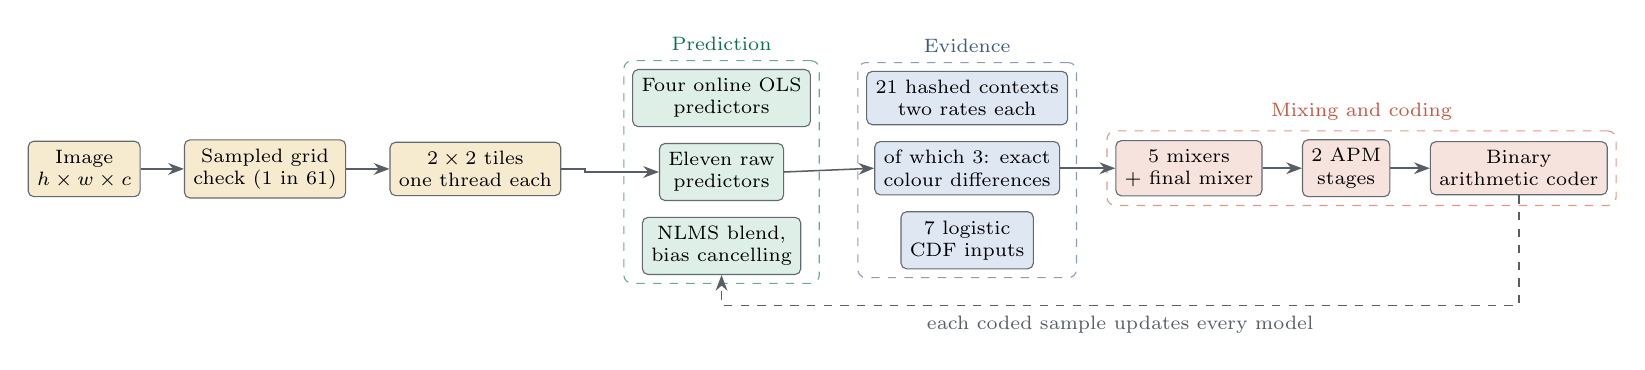
\begin{tikzpicture}[node distance=4mm and 5.5mm]
\node[box=softgold] (image) {Image\\$h\times w\times c$};
\node[box=softgold, right=of image] (gate) {Sampled grid\\check (1 in 61)};
\node[box=softgold, right=of gate] (tiles) {$2\times2$ tiles\\one thread each};
\node[box=softgreen, right=9mm of tiles, yshift=9mm] (ols) {Four online OLS\\predictors};
\node[box=softgreen, below=2mm of ols] (raw) {Eleven raw\\predictors};
\node[box=softgreen, below=2mm of raw] (blend) {NLMS blend,\\bias cancelling};
\node[box=softblue, right=7mm of ols] (ctx) {21 hashed contexts\\two rates each};
\node[box=softblue, below=2mm of ctx] (exact) {of which 3: exact\\colour differences};
\node[box=softblue, below=2mm of exact] (par) {7 logistic\\CDF inputs};
\node[box=softred, right=7mm of exact] (mix) {5 mixers\\+ final mixer};
\node[box=softred, right=5mm of mix] (apm) {2 APM\\stages};
\node[box=softred, right=5mm of apm] (ac) {Binary\\arithmetic coder};
\begin{scope}[on background layer]
\node[draw=ours!60, dashed, rounded corners=3pt, inner sep=3pt, fit=(ols)(raw)(blend), label={[font=\scriptsize,ours]above:Prediction}] {};
\node[draw=third!60, dashed, rounded corners=3pt, inner sep=3pt, fit=(ctx)(exact)(par), label={[font=\scriptsize,third]above:Evidence}] {};
\node[draw=rival!60, dashed, rounded corners=3pt, inner sep=3pt, fit=(mix)(apm)(ac), label={[font=\scriptsize,rival]above:Mixing and coding}] {};
\end{scope}
\draw[flow] (image) -- (gate);
\draw[flow] (gate) -- (tiles);
\draw[flow] (tiles.east) -- ++(3mm,0) |- (raw.west);
\draw[flow] (raw.east) -- (exact.west);
\draw[flow] (exact.east) -- (mix.west);
\draw[flow] (mix) -- (apm);
\draw[flow] (apm) -- (ac);
\draw[flow, dashed] (ac.south) -- ++(0,-14mm) -| node[pos=0.25,below,font=\scriptsize] {each coded sample updates every model} (blend.south);
\end{tikzpicture}}
\caption{Truepix. Each tile is coded independently and each sample is broken into binary decisions, as in Figure~\ref{fig:tree}.}
\label{fig:arch}
\end{figure*}

\subsection{Prediction}

Four recursive least-squares predictors run per plane. Each keeps an exponentially weighted covariance and solves by Cholesky factorisation every few samples:
\begin{equation}
\mathbf{R}_t=\lambda\mathbf{R}_{t-1}+(1-\lambda)\mathbf{x}_t\mathbf{x}_t^\top,\quad
\mathbf{w}_t=(\mathbf{R}_t+\nu\mathbf{I})^{-1}\mathbf{r}_t.
\end{equation}
Table~\ref{tab:ols} gives their settings. Regressors include causal neighbours in earlier planes, including the current pixel. Later planes keep a separate solver for each $2\times2$ position, because subsampled chroma behaves differently by phase.

\begin{table}[t]
\centering\small
\caption{Least-squares predictors. ``Own'' counts neighbours in the same plane, and ``cross-plane'' counts neighbours per earlier plane, before removing any that are not yet decoded.}
\label{tab:ols}
\setlength{\tabcolsep}{5pt}
\begin{tabular}{@{}lcccc@{}}
\toprule
Predictor & Own & Cross-plane & $\lambda$ & Solve every\\
\midrule
Standard & 18 & 7 & 0.9985 & 16\\
Medium & 10 & 4 & 0.995 & 8\\
Fast & 5 & 2 & 0.97 & 4\\
Wide & 30 & 7 & 0.9995 & 32\\
\bottomrule
\end{tabular}
\end{table}

Three of these join simple predictors (median edge, neighbours, gradient and inter-plane forms) and a combination weighted by each predictor's recent local error, giving eleven raw predictions. A normalised LMS blend, chosen by local activity, merges them into $\hat{x}$, followed by context-based bias cancellation.

\subsection{Binary decomposition}

The rounded prediction $P$ splits each sample into a short series of decisions (Figure~\ref{fig:tree}). Keeping $P$ as the origin concentrates statistics, and each decision can be priced directly by a parametric distribution as well as learned by counters.

\begin{figure}[t]
\centering
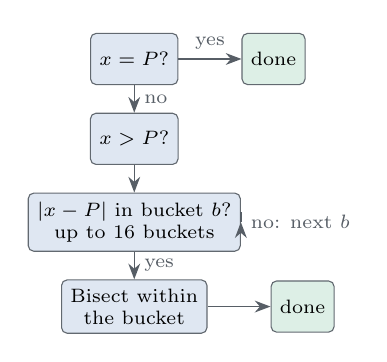
\begin{tikzpicture}[node distance=3.5mm and 3.5mm, every node/.style={font=\scriptsize}]
\node[box=softblue] (z) {$x=P$?};
\node[box=softgreen, right=8mm of z] (done) {done};
\node[box=softblue, below=of z] (s) {$x>P$?};
\node[box=softblue, below=of s] (b) {$|x-P|$ in bucket $b$?\\up to 16 buckets};
\node[box=softblue, below=of b] (m) {Bisect within\\the bucket};
\node[box=softgreen, right=8mm of m] (done2) {done};
\draw[flow] (z) -- node[above]{yes} (done);
\draw[flow] (z) -- node[right]{no} (s);
\draw[flow] (s) -- (b);
\draw[flow] (b) -- node[right]{yes} (m);
\draw[flow] (b.east) to[out=25,in=-25,looseness=5] node[right]{no: next $b$} (b.east);
\draw[flow] (m) -- (done2);
\end{tikzpicture}
\caption{Decisions for one sample. Range limits skip decisions that are already certain.}
\label{fig:tree}
\end{figure}

\subsection{Exact-difference contexts}
\label{sec:exact}

A decision's meaning depends on $P$, so a context that omits $P$ cannot learn that specific sample values are impossible. The fix is to include the difference between $P$ and the already coded sample $G$, exactly and unquantised. Writing $d=P-G$, a counter at residual node $n$ then refers to one definite value of $x-G$, and can learn which differences occur. For plane index $i$, with $k$ the known difference $R-G$ when coding $B$:
\begin{align}
c_{1}&=h(i,d,k),\notag\\
c_{2}&=h(i,d,k,\,W-W_G),\notag\\
c_{3}&=h(i,d,k,\,W-W_G,\,N-N_G),
\end{align}
where $W$, $N$ are this plane's neighbours and $W_G$, $N_G$ their green samples. No lattice is detected or fitted. On \texttt{kodim01} coded without mode~2, this and the smaller changes of Table~\ref{tab:ablation} together took blue from 2.07 to \plaz\ bits per pixel and red from 2.22 to \plax. For Kodak that is less than mode~2 achieves (Table~\ref{tab:planes}), but it also works where no formula is known.

That matters because such structure is common. In 16 unlocked DIV2K images the same recovered bases recurred across unrelated photographs, for example $(4.49,-3.0)$ and $(-1.0,-6.15)$ in eight images, and $(0.45,2.74)$ and $(4.83,-0.96)$ in three. We have not established where they come from, and they do not all match standard transforms. Fitting formulas image by image looked fragile, and learning sidesteps the question.

\begin{table}[t]
\centering\small
\caption{Cost of \texttt{kodim01}'s planes, in bits per pixel. Mode~2 also pays for corrections, omitted here, which bring its total to 6.42.}
\label{tab:planes}
\begin{tabular}{@{}lccc@{}}
\toprule
Version & First plane & Second & Third\\
\midrule
Before this work & 5.06 & 2.22 & 2.07\\
Final model, plain RGB & \play & \plax & \plaz\\
Mode 2, on $(Y,c_1,c_2)$ & \plcx & \plcy & \plcz\\
\bottomrule
\end{tabular}
\end{table}

\subsection{Mixing}

The 21 contexts each feed fast and slow adaptive counters, stored in tables of $2^{19}$ entries. With seven parametric logistic inputs and a bias, each decision has 50 inputs in the logit domain. Five mixers, selected by decision node combined with activity, gradient, position and local texture, feed a final mixer. Two adaptive probability maps refine the output, which drives a 32-bit binary arithmetic coder with 16-bit probabilities.

\subsection{Grid modes}

Mode~1 inverts the libjpeg YCbCr conversion, and mode~2 inverts Eq.~\ref{eq:fixed}. The encoder tests one pixel in 61 and skips the expensive inversion unless at least half fit. If at least 60\% of all pixels fit, it encodes that mode as well and keeps the smaller result. Corrections are coded with a small adaptive model after the planes.

\subsection{Tiles}

Images of one megapixel or more are split into $2\times2$ independently coded tiles on separate threads. Tiles are the only source of parallelism, and they lose context across boundaries. Figure~\ref{fig:tiles} shows the trade-off: two tiles per side cost \tilecosttwo\% and run \tilefactor\ times faster, while beyond four per side nothing more is gained on this eight-core machine.

\begin{figure}[t]
\centering
\resizebox{\columnwidth}{!}{%
\begin{tikzpicture}
\begin{axis}[width=\columnwidth, height=42mm, xlabel={Tiles per side}, ylabel={Encode time (s)}, xtick={1,2,3,4,6}, ymin=0, ymax=55, axis y line*=left, ylabel style={ours}, ymajorgrids, grid style={ink!12}]
\addplot[ours, line width=0.9pt, mark=*, mark size=1.3pt] table[x=side,y=time] {data/tiles.dat};
\end{axis}
\begin{axis}[width=\columnwidth, height=42mm, xtick=\empty, ylabel={Size cost (\%)}, ymin=0, ymax=2, axis y line*=right, axis x line=none, ylabel style={rival}]
\addplot[rival, line width=0.9pt, mark=square*, mark size=1.2pt, dashed] table[x=side,y=cost] {data/tiles.dat};
\end{axis}
\end{tikzpicture}}
\caption{Tile count against mean encode time (solid) and total size (dashed) on six unlocked images.}
\label{fig:tiles}
\end{figure}

\section{Reproducible floating point}
\label{sec:portable}

A symmetric codec fails silently if encoder and decoder disagree in one low-order bit. Fixed point is the usual remedy, but IEEE~754 requires addition, subtraction, multiplication, division and square root to be correctly rounded \cite{ieee}. Reproducibility then needs only that the program's operations are the same everywhere \cite{monniaux}. Three things had to change:

\begin{enumerate}\setlength\itemsep{1pt}\setlength\parskip{0pt}
\item \textbf{No libm.} \texttt{log} and \texttt{exp} are replaced by polynomial versions built only from the operations above.
\item \textbf{Fixed summation order.} Mixer dot products accumulate in eight lanes with a fixed final tree, so vector width cannot alter the sum, and the compiler can still vectorise it.
\item \textbf{No contraction.} \texttt{-ffp-contract=off} stops multiply-add fusion. Compile-time checks refuse \texttt{-ffast-math} and excess-precision targets. The contraction flag itself cannot be checked in the source, so it remains a build requirement.
\end{enumerate}

The file (Figure~\ref{fig:format}) stores a CRC-32 of the pixels, so a disagreement is an error rather than a wrong image. Every tile header is validated against the file header before any model is allocated, which closes a memory-safety hole for untrusted files.

\begin{figure}[t]
\centering
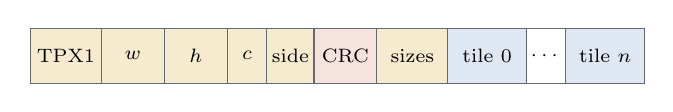
\begin{tikzpicture}[x=1mm,y=1mm, every node/.style={font=\scriptsize}]
\foreach \x/\w/\t/\c in {0/9/TPX1/softgold, 9/8/$w$/softgold, 17/8/$h$/softgold, 25/5/$c$/softgold, 30/6/side/softgold, 36/8/CRC/softred, 44/9/sizes/softgold, 53/10/tile 0/softblue, 63/5/$\cdots$/white, 68/10/tile $n$/softblue}{
  \draw[fill=\c, draw=ink!70] (\x,0) rectangle ++(\w,7);
  \node at (\x+\w/2,3.5) {\t};
}
\end{tikzpicture}
\caption{\texttt{TPX1} layout. Each tile repeats its own size and mode, and is checked before decoding.}
\label{fig:format}
\end{figure}

\paragraph{Evidence.}
We built seven ways: GCC~14 with AVX2, with FMA enabled, with baseline SSE2, and unoptimised; Clang (via Zig) for 64-bit and 32-bit x86; and WebAssembly under Node. Five test images covered plain RGB, Photo~CD, JPEG history, greyscale and RGBA. Every build wrote byte-identical files, and every build decoded every other build's file exactly: all $7\times7\times5=\matrixdecodes$ decodes (Figure~\ref{fig:matrix}). In a separate check, a full-size tiled image also matched across GCC, Clang, 32-bit x86 and WebAssembly. All 12 random bit flips in a coded stream were rejected, and no wrong image was returned. ARM64 compiles but has never been run, so that case remains untested.

\begin{figure}[t]
\centering
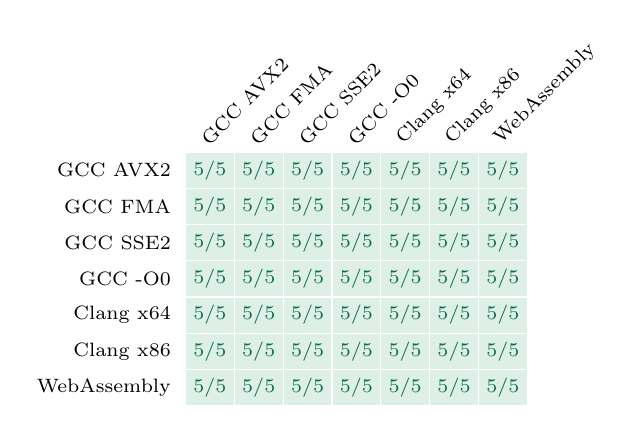
\begin{tikzpicture}[x=6.2mm,y=4.6mm, every node/.style={font=\scriptsize}]
\def\names{{"GCC AVX2","GCC FMA","GCC SSE2","GCC -O0","Clang x64","Clang x86","WebAssembly"}}
\foreach \i in {0,...,6}{
  \pgfmathsetmacro{\n}{\names[\i]}
  \node[anchor=east] at (-0.1,-\i-0.5) {\n};
  \node[anchor=west,rotate=45] at (\i+0.25,0.1) {\n};
  \foreach \j in {0,...,6}{
    \draw[fill=softgreen, draw=white] (\j,-\i) rectangle ++(1,-1);
    \node[ours] at (\j+0.5,-\i-0.5) {5/5};
  }
}
\end{tikzpicture}
\caption{Row build decoding column build's files. Each cell counts exact decodes out of five images.}
\label{fig:matrix}
\end{figure}

\section{Method}

\paragraph{Data.}
Three kinds of set were kept apart. \emph{Design:} 17 PNGs used to build the codec, and Kodak once it was studied. \emph{Tuning:} crops of DIV2K validation images 0825--0840 \cite{div2k}. \emph{Hold-out:} three blocks of 24 consecutive DIV2K images, chosen by filename rule before being opened, each checksummed and scored once by a frozen codec: Set~A (0801--0824), Set~B (0841--0864) and Set~C (0865--0888). Only Set~C is scored by the final build, and it is our primary result. Set~B was scored by the tiled build before the portability changes. Set~A was first scored without tiles, at a lead of 4.55\% over JPEG~XL effort~10 and 24 of 24 wins, then rerun with tiles for Table~\ref{tab:holdout}.

\paragraph{Verification.}
All Truepix results were decoded and compared byte for byte, and rival results were decoded and compared where they are reported. Rivals used their strongest lossless settings: JPEG~XL efforts 9 and 10, FLIF \texttt{-E100}, WebP method~6.

\paragraph{Statistics.}
Paired by image, we report total size, a percentile bootstrap (20,000 resamples of images) for the geometric-mean ratio, and an exact Wilcoxon signed-rank test.

\paragraph{Timing.}
A Ryzen~7 5800HS (8 cores, 16 threads, 15\,GB) ran one job at a time, with each library's default threading. The machine was not idle throughout: an unrelated CPU job shared it for part of the work, so timings are indicative. Paq8px was too slow to run on the hold-out sets.

\section{Results}
\label{sec:results}

\subsection{Compression}

Table~\ref{tab:holdout} gives the main results. On Set~C, Truepix is smaller than every rival on all 24 images. Against JPEG~XL at effort~10 the total lead is \setCtengain\% and the geometric-mean lead \cgeo\% (95\% CI [\cgeolo, \cgeohi]), ranging from \cminsave\% to \cmaxsave\% by image (Figure~\ref{fig:savings}). The signed-rank test gives $p=1.2\times10^{-7}$, the smallest value possible with 24 pairs. The leads on Sets~A and~B were \setAtengain\% and \setBtengain\%, so a fair summary is 3.6--4.3\%. Tiling cost one win on Set~A: image 0804 moved from a narrow win to a 0.16\% loss.

\begin{table*}[t]
\centering\small
\caption{Hold-out results. Each set is 24 images of about 2.8 megapixels. ``Bigger'' compares total size with Truepix on that set, and ``wins'' counts images where Truepix is smaller. All Truepix files decoded exactly. Set~A is shown with tiles, and Set~C alone used the final build.}
\label{tab:holdout}
\begin{tabular}{@{}l rrr rrr rrr@{}}
\toprule
& \multicolumn{3}{c}{Set A (0801--0824)} & \multicolumn{3}{c}{Set B (0841--0864)} & \multicolumn{3}{c}{\textbf{Set C (0865--0888), final build}}\\
\cmidrule(lr){2-4}\cmidrule(lr){5-7}\cmidrule(l){8-10}
Method & bpp & bigger & wins & bpp & bigger & wins & bpp & bigger & wins\\
\midrule
\textbf{Truepix} & \textbf{\setAbpp} & -- & -- & \textbf{\setBbpp} & -- & -- & \textbf{\setCbpp} & -- & --\\
JPEG XL, effort 10 & \setAtenbpp & \setAtengain\% & \setAtenwins/24 & \setBtenbpp & \setBtengain\% & \setBtenwins/24 & \setCtenbpp & \setCtengain\% & \setCtenwins/24\\
JPEG XL, effort 9 & \setAninebpp & \setAninegain\% & \setAninewins/24 & \setBninebpp & \setBninegain\% & \setBninewins/24 & \setCninebpp & \setCninegain\% & \setCninewins/24\\
FLIF & \setAflifbpp & \setAflifgain\% & \setAflifwins/24 & \setBflifbpp & \setBflifgain\% & \setBflifwins/24 & \setCflifbpp & \setCflifgain\% & \setCflifwins/24\\
WebP lossless & \setAwebpbpp & \setAwebpgain\% & \setAwebpwins/24 & \setBwebpbpp & \setBwebpgain\% & \setBwebpwins/24 & \setCwebpbpp & \setCwebpgain\% & \setCwebpwins/24\\
PNG as distributed & \setApngbpp & \setApnggain\% & \setApngwins/24 & \setBpngbpp & \setBpnggain\% & \setBpngwins/24 & \setCpngbpp & \setCpnggain\% & \setCpngwins/24\\
\bottomrule
\end{tabular}
\end{table*}

\begin{figure}[t]
\centering
\begin{tikzpicture}
\begin{axis}[width=\columnwidth, height=40mm, ybar, bar width=4.2pt, xlabel={Set C images, sorted}, ylabel={Saving (\%)}, ymin=0, xmin=0, xmax=25, xtick=\empty, ymajorgrids, grid style={ink!12}]
\addplot[fill=ours!75, draw=none] table[x=rank,y=saving] {data/savings.dat};
\end{axis}
\end{tikzpicture}
\caption{Truepix's size saving against JPEG~XL at effort~10, per image.}
\label{fig:savings}
\end{figure}

On the design PNGs, Truepix totals \dfinal\ bytes, \dbestgain\% below \dbestname\ (smaller on \dbestwins\ of 17). On Kodak it totals \kfinal\ bytes. Table~\ref{tab:kodakfield} lists Kodak rivals, but these figures show Photo~CD history, not general strength, and they should not be read as a fair score.

\begin{table}[t]
\centering\small
\caption{Kodak (design set, not a fair score). Truepix: \kfinal\ bytes, \kfinalbpp\ bpp. paq8px: \kpaq\ bytes.}
\label{tab:kodakfield}
\begin{tabular}{@{}lrrrr@{}}
\toprule
Method & Bytes & bpp & Bigger & Wins\\
\midrule
\rawinput data/kodak_field.tex
\bottomrule
\end{tabular}
\end{table}

\subsection{Against paq8px}

We could only compare paq8px on the 16 tuning crops, where the final Truepix is still behind: green 2,697,523 against 2,566,223 bytes (paq8px 4.9\% smaller), colour 5,638,301 against 5,267,444 (6.6\% smaller). Truepix is therefore not the strongest compressor here, and cmix, GraLIC, EMMA and learned codecs \cite{l3c} were not tested at all.

\subsection{What helped, and what did not}

Table~\ref{tab:ablation} records each change in turn. Gains were modest except for exact-difference contexts, and several reasonable ideas failed. Trying several spreads per sample did nothing. Pre-training was estimated by stacking one image above another: the second image saved about 0.8\%, too little to justify. Learning rates were already near their best. A green gap of about 5\% to paq8px remains and has not been explained.

\begin{table}[t]
\centering\small
\caption{Development steps on 16 tuning crops (cumulative bytes). Rejected steps were removed before continuing.}
\label{tab:ablation}
\begin{tabular}{@{}p{46mm}rr@{}}
\toprule
Step & Green & Colour\\
\midrule
Starting point & 2,718,580 & 5,730,204\\
Several spreads (rejected) & 2,720,159 & --\\
Wide OLS, local weighting & 2,712,692 & --\\
Texture contexts, fifth mixer & 2,700,742 & --\\
Exact-difference contexts & -- & 5,645,837\\
Neighbour pairs (rejected) & -- & 5,640,271\\
Final build, all kept changes & 2,697,523 & 5,638,301\\
\midrule
paq8px, for reference & 2,566,223 & 5,267,444\\
\bottomrule
\end{tabular}
\end{table}

\subsection{Speed}

Table~\ref{tab:speed} and Figure~\ref{fig:speed} give timing on five Set~C images. Encoding with tiles takes about \sppxmtwoenc\,s, between JPEG~XL at effort~9 (\spjxlnineenc\,s) and effort~10 (\spjxltenenc\,s). Decoding is Truepix's real weakness: \sppxmtwodec\,s against \spjxlninedec\,s, about \decodegap\ times slower, because a symmetric model does all its work again. Truepix suits archiving, not web delivery. By calculation, the tables of a tiled image take about 265\,MB.

\begin{table}[t]
\centering\small
\caption{Mean seconds per image on five Set~C images (2.8\,MP on average), with total size against Truepix with $2\times2$ tiles.}
\label{tab:speed}
\begin{tabular}{@{}lrrr@{}}
\toprule
Method & Encode & Decode & Size\\
\midrule
\rawinput data/speed.tex
\bottomrule
\end{tabular}
\end{table}

\begin{figure}[t]
\centering
\begin{tikzpicture}
\begin{axis}[width=\columnwidth, height=47mm, xmode=log, xlabel={Mean decode time (s, log scale)}, ylabel={Size vs Truepix $2\times2$ (\%)}, ymin=-3, ymax=24, xmin=0.03, xmax=90, ymajorgrids, xmajorgrids, grid style={ink!12},
  every node near coord/.style={font=\scriptsize, anchor=west, xshift=1pt, text=ink}]
\addplot[only marks, mark=*, mark size=1.5pt, rival, nodes near coords, point meta=explicit symbolic] table[x=dec,y=rel,meta=label] {data/speed_rivals.dat};
\addplot[only marks, mark=*, mark size=1.7pt, ours] table[x=dec,y=rel] {data/speed_pxm.dat};
\node[ours, font=\scriptsize, anchor=south] at (axis cs:11,1.6) {Truepix: $4{\times}4$, $2{\times}2$, whole};
\end{axis}
\end{tikzpicture}
\caption{Size against decode time. Lower left is better. Truepix's lead is bought with roughly two orders of magnitude in decode time.}
\label{fig:speed}
\end{figure}

\section{Discussion}

\paragraph{What is and is not shown.}
Our claim is narrow: among the practical codecs tested, on these DIV2K images, Truepix gave the smallest files, by about 3.6--4.3\% over JPEG~XL's top effort. DIV2K may not represent all photographs, and these sets come from one source. All hold-out sets are now used, though 12 of the 100 DIV2K validation images remain unseen.

\paragraph{Limits of the method.}
The Photo~CD form was fitted to Kodak itself, not to independent Photo~CD scans, and the rest of its misses are unexplained. Our literature search was limited. Truepix handles only 8-bit images, and cannot reproduce JPEG files byte for byte, for which JPEG~XL transcoding remains the right tool.

\paragraph{Future work.}
Decode speed is the priority, likely through cheaper counters and fewer mixer inputs. Chroma subsampling is visible in mode~2's position-dependent costs (\plcyA, \plcyB, \plcyC\ and \plcyD\ bits per sample in the second plane, by position), but is not yet explicitly modelled. The recurring DIV2K lattices need an explanation, and the remaining green gap to paq8px is the largest open compression question. ARM execution must also be tested.

\section{Conclusion}

The surprising strength of a slow compressor on a famous benchmark was not a matter of better modelling alone. It was the benchmark's history: an integer colour lattice from Photo~CD, recoverable from pixels and matching constants Kodak published decades ago. Turning that observation into exact-difference contexts yields a practical gain with no history detection at all. Truepix's lead over JPEG~XL held across three unseen sets, reproducibly across seven builds, at the stated cost in decode time.

\paragraph{Reproducibility.}
Results were measured as PXM, the name in the raw files. The release differs from the scored build only in its name and file marker: on eight test images, its files matched byte for byte after that marker. The raw results, the script behind this paper's numbers and plots, and the measurement scripts are in \texttt{paper/}. Hard-coded development figures in Tables~\ref{tab:ablation} and~\ref{tab:planes} and Figure~\ref{fig:gap} come from the session logs. Independent replication has not been attempted.

\paragraph{Acknowledgement.}
Implementation, experiments and drafting were carried out with Claude Code, an AI coding assistant.

\small
\balance
\begin{thebibliography}{99}\setlength\itemsep{1pt}
\bibitem{jpegxl} J.~Alakuijala et al., ``JPEG XL next-generation image compression architecture and coding tools,'' in \emph{Proc. SPIE Applications of Digital Image Processing XLII}, 2019.
\bibitem{mahoney} M.~Mahoney, ``Adaptive weighing of context models for lossless data compression,'' Florida Tech. Tech. Rep. CS-2005-16, 2005.
\bibitem{paq8px} paq8px contributors, \emph{paq8px}, version 217 used here, \url{https://github.com/hxim/paq8px}.
\bibitem{kodak} R.~Franzen, ``Kodak lossless true color image suite,'' \url{https://r0k.us/graphics/kodak/}.
\bibitem{jpegls} M.~J.~Weinberger, G.~Seroussi, and G.~Sapiro, ``The LOCO-I lossless image compression algorithm: principles and standardization into JPEG-LS,'' \emph{IEEE Trans. Image Process.}, vol.~9, no.~8, 2000.
\bibitem{calic} X.~Wu and N.~Memon, ``Context-based, adaptive, lossless image coding,'' \emph{IEEE Trans. Commun.}, vol.~45, no.~4, 1997.
\bibitem{edp} X.~Li and M.~T.~Orchard, ``Edge-directed prediction for lossless compression of natural images,'' \emph{IEEE Trans. Image Process.}, vol.~10, no.~6, 2001.
\bibitem{tmw} B.~Meyer and P.~Tischer, ``TMW --- a new method for lossless image compression,'' in \emph{Proc. Picture Coding Symp.}, 1997.
\bibitem{mrp} I.~Matsuda, N.~Ozaki, Y.~Umezu, and S.~Itoh, ``Lossless coding using variable block-size adaptive prediction optimized for each image,'' in \emph{Proc. EUSIPCO}, 2005.
\bibitem{vanilc} A.~Weinlich, P.~Amon, A.~Hutter, and A.~Kaup, ``Probability distribution estimation for autoregressive pixel-predictive image coding,'' \emph{IEEE Trans. Image Process.}, vol.~25, no.~3, 2016.
\bibitem{flif} J.~Sneyers and P.~Wuille, ``FLIF: Free lossless image format based on MANIAC compression,'' in \emph{Proc. IEEE ICIP}, 2016.
\bibitem{l3c} F.~Mentzer, E.~Agustsson, M.~Tschannen, R.~Timofte, and L.~Van~Gool, ``Practical full resolution learned lossless image compression,'' in \emph{Proc. IEEE/CVF CVPR}, 2019.
\bibitem{fan} Z.~Fan and R.~L.~de~Queiroz, ``Identification of bitmap compression history: JPEG detection and quantizer estimation,'' \emph{IEEE Trans. Image Process.}, vol.~12, no.~2, 2003.
\bibitem{neelamani} R.~Neelamani, R.~de~Queiroz, Z.~Fan, S.~Dash, and R.~G.~Baraniuk, ``JPEG compression history estimation for color images,'' \emph{IEEE Trans. Image Process.}, vol.~15, no.~6, 2006.
\bibitem{lewis} A.~B.~Lewis and M.~G.~Kuhn, ``Exact JPEG recompression,'' in \emph{Proc. SPIE Visual Information Processing and Communication}, 2010.
\bibitem{monniaux} D.~Monniaux, ``The pitfalls of verifying floating-point computations,'' \emph{ACM Trans. Program. Lang. Syst.}, vol.~30, no.~3, 2008.
\bibitem{ieee} \emph{IEEE Standard for Floating-Point Arithmetic}, IEEE Std 754-2019.
\bibitem{pcd045} Eastman Kodak Company, ``Fully utilizing Photo CD images, article no.~4: PhotoYCC color encoding and compression schemes,'' Photo CD Information Bulletin PCD 045, 1994.
\bibitem{div2k} E.~Agustsson and R.~Timofte, ``NTIRE 2017 challenge on single image super-resolution: dataset and study,'' in \emph{Proc. IEEE CVPR Workshops}, 2017.
\end{thebibliography}
\end{document}
